% Options for packages loaded elsewhere
\PassOptionsToPackage{unicode}{hyperref}
\PassOptionsToPackage{hyphens}{url}
\PassOptionsToPackage{dvipsnames,svgnames,x11names}{xcolor}
%
\documentclass[
  11pt,
  a4paper,
]{article}

\usepackage{amsmath,amssymb}
\usepackage{setspace}
\usepackage{iftex}
\ifPDFTeX
  \usepackage[T1]{fontenc}
  \usepackage[utf8]{inputenc}
  \usepackage{textcomp} % provide euro and other symbols
\else % if luatex or xetex
  \usepackage{unicode-math}
  \defaultfontfeatures{Scale=MatchLowercase}
  \defaultfontfeatures[\rmfamily]{Ligatures=TeX,Scale=1}
\fi
\usepackage{lmodern}
\ifPDFTeX\else  
    % xetex/luatex font selection
    \setmainfont[]{Times New Roman}
    \setsansfont[]{Arial}
    \setmonofont[]{Courier New}
\fi
% Use upquote if available, for straight quotes in verbatim environments
\IfFileExists{upquote.sty}{\usepackage{upquote}}{}
\IfFileExists{microtype.sty}{% use microtype if available
  \usepackage[]{microtype}
  \UseMicrotypeSet[protrusion]{basicmath} % disable protrusion for tt fonts
}{}
\makeatletter
\@ifundefined{KOMAClassName}{% if non-KOMA class
  \IfFileExists{parskip.sty}{%
    \usepackage{parskip}
  }{% else
    \setlength{\parindent}{0pt}
    \setlength{\parskip}{6pt plus 2pt minus 1pt}}
}{% if KOMA class
  \KOMAoptions{parskip=half}}
\makeatother
\usepackage{xcolor}
\usepackage[margin=2.5cm]{geometry}
\setlength{\emergencystretch}{3em} % prevent overfull lines
\setcounter{secnumdepth}{3}
% Make \paragraph and \subparagraph free-standing
\makeatletter
\ifx\paragraph\undefined\else
  \let\oldparagraph\paragraph
  \renewcommand{\paragraph}{
    \@ifstar
      \xxxParagraphStar
      \xxxParagraphNoStar
  }
  \newcommand{\xxxParagraphStar}[1]{\oldparagraph*{#1}\mbox{}}
  \newcommand{\xxxParagraphNoStar}[1]{\oldparagraph{#1}\mbox{}}
\fi
\ifx\subparagraph\undefined\else
  \let\oldsubparagraph\subparagraph
  \renewcommand{\subparagraph}{
    \@ifstar
      \xxxSubParagraphStar
      \xxxSubParagraphNoStar
  }
  \newcommand{\xxxSubParagraphStar}[1]{\oldsubparagraph*{#1}\mbox{}}
  \newcommand{\xxxSubParagraphNoStar}[1]{\oldsubparagraph{#1}\mbox{}}
\fi
\makeatother

\usepackage{color}
\usepackage{fancyvrb}
\newcommand{\VerbBar}{|}
\newcommand{\VERB}{\Verb[commandchars=\\\{\}]}
\DefineVerbatimEnvironment{Highlighting}{Verbatim}{commandchars=\\\{\}}
% Add ',fontsize=\small' for more characters per line
\usepackage{framed}
\definecolor{shadecolor}{RGB}{241,243,245}
\newenvironment{Shaded}{\begin{snugshade}}{\end{snugshade}}
\newcommand{\AlertTok}[1]{\textcolor[rgb]{0.68,0.00,0.00}{#1}}
\newcommand{\AnnotationTok}[1]{\textcolor[rgb]{0.37,0.37,0.37}{#1}}
\newcommand{\AttributeTok}[1]{\textcolor[rgb]{0.40,0.45,0.13}{#1}}
\newcommand{\BaseNTok}[1]{\textcolor[rgb]{0.68,0.00,0.00}{#1}}
\newcommand{\BuiltInTok}[1]{\textcolor[rgb]{0.00,0.23,0.31}{#1}}
\newcommand{\CharTok}[1]{\textcolor[rgb]{0.13,0.47,0.30}{#1}}
\newcommand{\CommentTok}[1]{\textcolor[rgb]{0.37,0.37,0.37}{#1}}
\newcommand{\CommentVarTok}[1]{\textcolor[rgb]{0.37,0.37,0.37}{\textit{#1}}}
\newcommand{\ConstantTok}[1]{\textcolor[rgb]{0.56,0.35,0.01}{#1}}
\newcommand{\ControlFlowTok}[1]{\textcolor[rgb]{0.00,0.23,0.31}{\textbf{#1}}}
\newcommand{\DataTypeTok}[1]{\textcolor[rgb]{0.68,0.00,0.00}{#1}}
\newcommand{\DecValTok}[1]{\textcolor[rgb]{0.68,0.00,0.00}{#1}}
\newcommand{\DocumentationTok}[1]{\textcolor[rgb]{0.37,0.37,0.37}{\textit{#1}}}
\newcommand{\ErrorTok}[1]{\textcolor[rgb]{0.68,0.00,0.00}{#1}}
\newcommand{\ExtensionTok}[1]{\textcolor[rgb]{0.00,0.23,0.31}{#1}}
\newcommand{\FloatTok}[1]{\textcolor[rgb]{0.68,0.00,0.00}{#1}}
\newcommand{\FunctionTok}[1]{\textcolor[rgb]{0.28,0.35,0.67}{#1}}
\newcommand{\ImportTok}[1]{\textcolor[rgb]{0.00,0.46,0.62}{#1}}
\newcommand{\InformationTok}[1]{\textcolor[rgb]{0.37,0.37,0.37}{#1}}
\newcommand{\KeywordTok}[1]{\textcolor[rgb]{0.00,0.23,0.31}{\textbf{#1}}}
\newcommand{\NormalTok}[1]{\textcolor[rgb]{0.00,0.23,0.31}{#1}}
\newcommand{\OperatorTok}[1]{\textcolor[rgb]{0.37,0.37,0.37}{#1}}
\newcommand{\OtherTok}[1]{\textcolor[rgb]{0.00,0.23,0.31}{#1}}
\newcommand{\PreprocessorTok}[1]{\textcolor[rgb]{0.68,0.00,0.00}{#1}}
\newcommand{\RegionMarkerTok}[1]{\textcolor[rgb]{0.00,0.23,0.31}{#1}}
\newcommand{\SpecialCharTok}[1]{\textcolor[rgb]{0.37,0.37,0.37}{#1}}
\newcommand{\SpecialStringTok}[1]{\textcolor[rgb]{0.13,0.47,0.30}{#1}}
\newcommand{\StringTok}[1]{\textcolor[rgb]{0.13,0.47,0.30}{#1}}
\newcommand{\VariableTok}[1]{\textcolor[rgb]{0.07,0.07,0.07}{#1}}
\newcommand{\VerbatimStringTok}[1]{\textcolor[rgb]{0.13,0.47,0.30}{#1}}
\newcommand{\WarningTok}[1]{\textcolor[rgb]{0.37,0.37,0.37}{\textit{#1}}}

\providecommand{\tightlist}{%
  \setlength{\itemsep}{0pt}\setlength{\parskip}{0pt}}\usepackage{longtable,booktabs,array}
\usepackage{calc} % for calculating minipage widths
% Correct order of tables after \paragraph or \subparagraph
\usepackage{etoolbox}
\makeatletter
\patchcmd\longtable{\par}{\if@noskipsec\mbox{}\fi\par}{}{}
\makeatother
% Allow footnotes in longtable head/foot
\IfFileExists{footnotehyper.sty}{\usepackage{footnotehyper}}{\usepackage{footnote}}
\makesavenoteenv{longtable}
\usepackage{graphicx}
\makeatletter
\newsavebox\pandoc@box
\newcommand*\pandocbounded[1]{% scales image to fit in text height/width
  \sbox\pandoc@box{#1}%
  \Gscale@div\@tempa{\textheight}{\dimexpr\ht\pandoc@box+\dp\pandoc@box\relax}%
  \Gscale@div\@tempb{\linewidth}{\wd\pandoc@box}%
  \ifdim\@tempb\p@<\@tempa\p@\let\@tempa\@tempb\fi% select the smaller of both
  \ifdim\@tempa\p@<\p@\scalebox{\@tempa}{\usebox\pandoc@box}%
  \else\usebox{\pandoc@box}%
  \fi%
}
% Set default figure placement to htbp
\def\fps@figure{htbp}
\makeatother

\usepackage{fvextra}
\DefineVerbatimEnvironment{Highlighting}{Verbatim}{breaklines=true,breakanywhere=true,commandchars=\\\{\}}
\makeatletter
\@ifpackageloaded{caption}{}{\usepackage{caption}}
\AtBeginDocument{%
\ifdefined\contentsname
  \renewcommand*\contentsname{Table of contents}
\else
  \newcommand\contentsname{Table of contents}
\fi
\ifdefined\listfigurename
  \renewcommand*\listfigurename{List of Figures}
\else
  \newcommand\listfigurename{List of Figures}
\fi
\ifdefined\listtablename
  \renewcommand*\listtablename{List of Tables}
\else
  \newcommand\listtablename{List of Tables}
\fi
\ifdefined\figurename
  \renewcommand*\figurename{Figure}
\else
  \newcommand\figurename{Figure}
\fi
\ifdefined\tablename
  \renewcommand*\tablename{Table}
\else
  \newcommand\tablename{Table}
\fi
}
\@ifpackageloaded{float}{}{\usepackage{float}}
\floatstyle{ruled}
\@ifundefined{c@chapter}{\newfloat{codelisting}{h}{lop}}{\newfloat{codelisting}{h}{lop}[chapter]}
\floatname{codelisting}{Listing}
\newcommand*\listoflistings{\listof{codelisting}{List of Listings}}
\makeatother
\makeatletter
\makeatother
\makeatletter
\@ifpackageloaded{caption}{}{\usepackage{caption}}
\@ifpackageloaded{subcaption}{}{\usepackage{subcaption}}
\makeatother
\makeatletter
\@ifpackageloaded{tcolorbox}{}{\usepackage[skins,breakable]{tcolorbox}}
\makeatother
\makeatletter
\@ifundefined{shadecolor}{\definecolor{shadecolor}{rgb}{.97, .97, .97}}{}
\makeatother
\makeatletter
\makeatother
\makeatletter
\ifdefined\Shaded\renewenvironment{Shaded}{\begin{tcolorbox}[sharp corners, boxrule=0pt, borderline west={3pt}{0pt}{shadecolor}, interior hidden, enhanced, frame hidden, breakable]}{\end{tcolorbox}}\fi
\makeatother

\usepackage{bookmark}

\IfFileExists{xurl.sty}{\usepackage{xurl}}{} % add URL line breaks if available
\urlstyle{same} % disable monospaced font for URLs
\hypersetup{
  pdftitle={Redes bayesianas multinomiales},
  pdfauthor={Oliver Arturo Casas Pontanillo \textbar{} A01645764; Erik Abraham Jajan Díaz \textbar{} A01644648; José Luis Santos Montaño \textbar{} A01781721},
  colorlinks=true,
  linkcolor={blue},
  filecolor={Maroon},
  citecolor={Blue},
  urlcolor={Blue},
  pdfcreator={LaTeX via pandoc}}


\title{Redes bayesianas multinomiales}
\author{Oliver Arturo Casas Pontanillo \textbar{} A01645764 \and Erik
Abraham Jajan Díaz \textbar{} A01644648 \and José Luis Santos Montaño
\textbar{} A01781721}
\date{2025-08-31}

\begin{document}
\maketitle

\renewcommand*\contentsname{Table of contents}
{
\hypersetup{linkcolor=}
\setcounter{tocdepth}{3}
\tableofcontents
}

\setstretch{1.5}
https://github.com/olivercasas17/MA2014\_Redes\_bayesianas\_multinomiales

\subsection{Abstract}\label{abstract}

Este estudio analiza patrones de movilidad urbana a partir de la
Encuesta Origen--Destino 2017 del INEGI utilizando redes bayesianas
multinomiales. El objetivo principal es modelar las dependencias entre
variables sociodemográficas, de transporte y de viaje para estimar
probabilidades condicionales relevantes en el análisis de movilidad. La
metodología consistió en la construcción de grafos acíclicos dirigidos
(DAG), uno basado en conocimiento previo y otro generado mediante el
algoritmo de hill climbing. Ambos modelos fueron evaluados con métricas
estadísticas como el Criterio de Información de Akaike (AIC) y el
Criterio de Información Bayesiano (BIC). Los resultados muestran que el
modelo aprendido con hill climbing obtuvo un mejor ajuste, por lo que se
utilizó para realizar inferencia probabilística mediante consultas
condicionales (queries). Los hallazgos permiten identificar, por
ejemplo, la influencia de la localidad y el propósito del viaje en la
elección del transporte, así como diferencias significativas en la
duración de los viajes según el tamaño de la localidad. En conclusión,
las redes bayesianas se muestran como una herramienta útil para explorar
y predecir patrones de movilidad en contextos urbanos complejos.

\subsection{Introducción}\label{introducciuxf3n}

El estudio de la movilidad urbana es un componente esencial para
comprender la dinámica de las ciudades y apoyar la toma de decisiones en
materia de planeación y políticas públicas. La Encuesta Origen--Destino
2017 proporciona información detallada sobre los hábitos de transporte
de la población en México, lo que abre la posibilidad de aplicar
enfoques estadísticos avanzados para modelar las relaciones entre
variables sociodemográficas, espaciales y de transporte.

En este trabajo se propone el uso de redes bayesianas multinomiales como
marco de análisis. Estas redes permiten representar relaciones de
dependencia entre variables categóricas a través de grafos acíclicos
dirigidos (DAG), ofreciendo no solo una estructura visual de dichas
relaciones, sino también la capacidad de realizar inferencias
probabilísticas bajo condiciones específicas.

La construcción del modelo se llevó a cabo de dos maneras: (1) mediante
el diseño de una estructura basada en conocimiento previo y (2)
utilizando un enfoque de aprendizaje automático con el algoritmo de hill
climbing. Posteriormente, ambos modelos fueron evaluados con criterios
de información (AIC y BIC) para seleccionar la estructura con mejor
desempeño. Una vez identificado el modelo más adecuado, se realizaron
consultas condicionales con el fin de explorar preguntas relevantes,
como la relación entre el propósito del viaje y el uso del transporte
público, o la influencia del tamaño de la localidad en la duración de
los viajes.

Este enfoque no solo permite identificar patrones empíricos en los
datos, sino también aportar una herramienta flexible para el análisis
probabilístico de la movilidad urbana.

\subsection{Metodología}\label{metodologuxeda}

El trabajo sigue un enfoque cuantitativo, de modelado estadistico y
probabilistico, utiizando redes bayesianas multinomiales para
representar relaciones de dependencia entre las variables seleccionadas
para resolver las queries.

A partir de las queries proporcionadas, se analizaron para determinar
que variables tendriamos que extraer de la base de datos de la encuesta
Origen-Destino 2017. Una vez seleccionadas estas variables, fueron
procesadas en -- para poder trabajar con estos datos. Se construyeron
dos gráficos acíclicos dirigidos, tambien conocidos como DAG, uno basado
en conocimiento previo y otro generado con un algoritmo de optimizacion.
Se compararon las dos DAGs usando metricas estadisticas y, realizando un
ajuste de parametros con la mejor de las dos, se calcularon las queries.

Las principales tecnicas empleadas para realizar este articulo fueron:\\
-Análisis de redes bayesianas, construyendo grafos acíclicos dirigidos
para modelar relaciones de dependencia entre variables categoricas\\
-Algoritmos de optimizacion, especificamente hill climbing, como
generador de una DAG\\
-Evaluacion de modelos, usando metodos estadisticos como el Criterio de
Informacion de AKaike y el Criterio de Informacion Bayesiano, AIC y BIC
por sus siglas en ingles.\\
-Inferencia probabilistica, consultas condicionales para estimar
probabilidades bajo evidencia

Los materiales utilizados para realizar este analisis fueron los
siguientes:\\
data.csv - los datos procesados\\
tviaje.csv y tsdem.csv - los datos preprocesados\\
eod\_2017\_csv.zip - El conjunto completo de datos de la encuensta
Origen-Destino 2017

Las herramientas que utilizamos fueron las siguientes:\\
Lenguaje de programacion R\\
Librerias: dplyr, bnlearn, Rgraphviz\\
Entorno de trabajo R Studio

\subsection{Aplicación}\label{aplicaciuxf3n}

\begin{Shaded}
\begin{Highlighting}[numbers=left,,]
\FunctionTok{library}\NormalTok{(bnlearn)}

\NormalTok{data }\OtherTok{=} \FunctionTok{read.csv}\NormalTok{(}\StringTok{"../data/data.csv"}\NormalTok{, }\AttributeTok{stringsAsFactors =} \ConstantTok{TRUE}\NormalTok{)}
\FunctionTok{head}\NormalTok{(data)}
\end{Highlighting}
\end{Shaded}

\begin{verbatim}
   sexo     tiempo transporte         dia proposito viajes localidad
1 mujer entre30y60    publico entreSemana   trabajo  pocos   pequeña
2 mujer    mayor60    publico entreSemana     hogar  pocos   pequeña
3 mujer    menor30       otro finDeSemana  convivir  pocos   pequeña
4 mujer    menor30    privado finDeSemana     hogar  pocos   pequeña
5 mujer entre30y60    publico entreSemana   trabajo  pocos   pequeña
6 mujer    mayor60    publico entreSemana     hogar  pocos   pequeña
\end{verbatim}

La base de datos que estamos utilizando cuenta con 7 columnas,
categorizadas de la siguiente manera\\
sexo: hombre y mujer\\
tiempo - Duracion total del viaje: entre30y60, mayor60 y
menor30\textbackslash{} transporte\\
Tipo de transporte utilizado: publico, privado y otro\\
dia - Dia en el que se realizo el viaje: entreSemana y finDeSemana\\
proposito - Proposito del viaje\textbackslash{} viajes - Cantidad de
viajes que realiza el hogar de la persona que realiza el viaje: pocos y
muchos\\
localidad - Tamano de la localidad donde se realiza el viaje: pequeña y
grande

Creacion de la Dag usando hill climbing

\begin{Shaded}
\begin{Highlighting}[numbers=left,,]
\NormalTok{dag }\OtherTok{=} \FunctionTok{empty.graph}\NormalTok{(}\AttributeTok{nodes =} \FunctionTok{c}\NormalTok{(}\StringTok{"sexo"}\NormalTok{, }\StringTok{"tiempo"}\NormalTok{, }\StringTok{"transporte"}\NormalTok{, }\StringTok{"dia"}\NormalTok{, }\StringTok{"proposito"}\NormalTok{, }\StringTok{"viajes"}\NormalTok{, }\StringTok{"localidad"}\NormalTok{))}
\end{Highlighting}
\end{Shaded}

\begin{Shaded}
\begin{Highlighting}[numbers=left,,]
\NormalTok{hc\_dag }\OtherTok{=} \FunctionTok{hc}\NormalTok{(data)}
\end{Highlighting}
\end{Shaded}

\begin{Shaded}
\begin{Highlighting}[numbers=left,,]
\FunctionTok{modelstring}\NormalTok{(hc\_dag)}
\end{Highlighting}
\end{Shaded}

\begin{verbatim}
[1] "[tiempo][transporte|tiempo][dia|tiempo:transporte][proposito|tiempo:transporte:dia][sexo|tiempo:transporte:proposito][viajes|tiempo:proposito][localidad|transporte:viajes]"
\end{verbatim}

\begin{Shaded}
\begin{Highlighting}[numbers=left,,]
\FunctionTok{graphviz.plot}\NormalTok{(hc\_dag, }\AttributeTok{shape =} \StringTok{"ellipse"}\NormalTok{)}
\end{Highlighting}
\end{Shaded}

\begin{verbatim}
Loading required namespace: Rgraphviz
\end{verbatim}

\pandocbounded{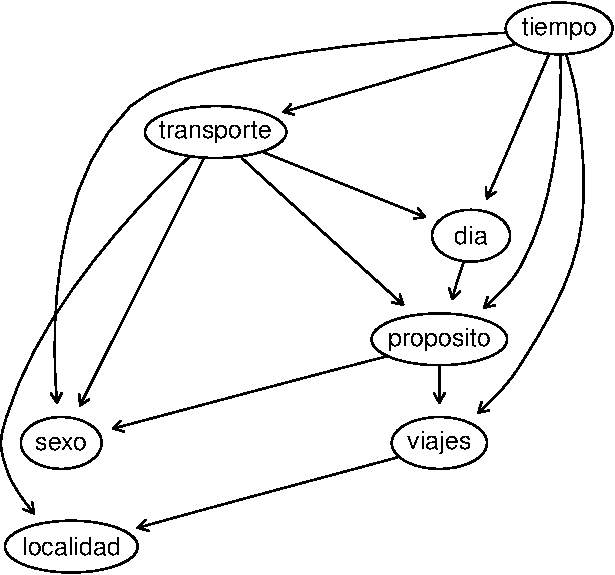
\includegraphics[keepaspectratio]{reporte_files/figure-pdf/unnamed-chunk-5-1.pdf}}

Evaluacion de la DAG creada

\begin{Shaded}
\begin{Highlighting}[numbers=left,,]
\FunctionTok{score}\NormalTok{(hc\_dag, }\AttributeTok{data =}\NormalTok{ data, }\AttributeTok{type =} \StringTok{"bic"}\NormalTok{)}
\end{Highlighting}
\end{Shaded}

\begin{verbatim}
[1] -2791118
\end{verbatim}

\begin{Shaded}
\begin{Highlighting}[numbers=left,,]
\FunctionTok{score}\NormalTok{(hc\_dag, }\AttributeTok{data =}\NormalTok{ data, }\AttributeTok{type =} \StringTok{"aic"}\NormalTok{)}
\end{Highlighting}
\end{Shaded}

\begin{verbatim}
[1] -2787909
\end{verbatim}

Creacion de la DAG utilizando conocimiento previo

\begin{Shaded}
\begin{Highlighting}[numbers=left,,]
\NormalTok{new\_dag }\OtherTok{=} \FunctionTok{empty.graph}\NormalTok{(}\AttributeTok{nodes =} \FunctionTok{c}\NormalTok{(}\StringTok{"sexo"}\NormalTok{, }\StringTok{"tiempo"}\NormalTok{, }\StringTok{"transporte"}\NormalTok{, }\StringTok{"dia"}\NormalTok{, }\StringTok{"proposito"}\NormalTok{, }\StringTok{"viajes"}\NormalTok{, }\StringTok{"localidad"}\NormalTok{))}
\end{Highlighting}
\end{Shaded}

\begin{Shaded}
\begin{Highlighting}[numbers=left,,]
\NormalTok{arc\_set }\OtherTok{=} \FunctionTok{matrix}\NormalTok{(}\FunctionTok{c}\NormalTok{(}\StringTok{"sexo"}\NormalTok{, }\StringTok{"proposito"}\NormalTok{,}
                   \StringTok{"sexo"}\NormalTok{, }\StringTok{"transporte"}\NormalTok{,}
                   \StringTok{"localidad"}\NormalTok{, }\StringTok{"transporte"}\NormalTok{,}
                   \StringTok{"proposito"}\NormalTok{, }\StringTok{"dia"}\NormalTok{,}
                   \StringTok{"transporte"}\NormalTok{, }\StringTok{"tiempo"}\NormalTok{,}
                   \StringTok{"localidad"}\NormalTok{, }\StringTok{"tiempo"}\NormalTok{,}
                   \StringTok{"dia"}\NormalTok{, }\StringTok{"viajes"}\NormalTok{,}
                   \StringTok{"tiempo"}\NormalTok{, }\StringTok{"viajes"}\NormalTok{), }\AttributeTok{byrow =} \ConstantTok{TRUE}\NormalTok{, }\AttributeTok{ncol =} \DecValTok{2}\NormalTok{,}
                 \AttributeTok{dimnames =} \FunctionTok{list}\NormalTok{(}\ConstantTok{NULL}\NormalTok{, }\FunctionTok{c}\NormalTok{(}\StringTok{"from"}\NormalTok{, }\StringTok{"to"}\NormalTok{)))}
\end{Highlighting}
\end{Shaded}

\begin{Shaded}
\begin{Highlighting}[numbers=left,,]
\FunctionTok{arcs}\NormalTok{(new\_dag) }\OtherTok{=}\NormalTok{ arc\_set}
\end{Highlighting}
\end{Shaded}

\begin{Shaded}
\begin{Highlighting}[numbers=left,,]
\FunctionTok{graphviz.plot}\NormalTok{(new\_dag, }\AttributeTok{shape =} \StringTok{"ellipse"}\NormalTok{)}
\end{Highlighting}
\end{Shaded}

\pandocbounded{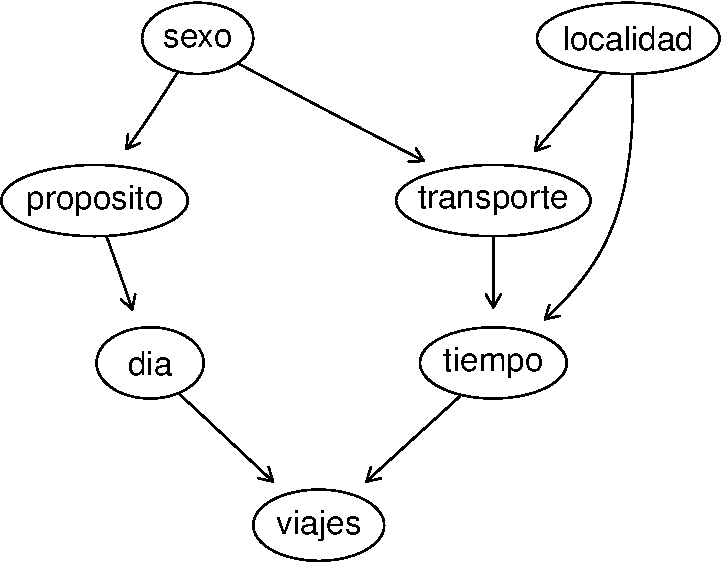
\includegraphics[keepaspectratio]{reporte_files/figure-pdf/unnamed-chunk-11-1.pdf}}

Evaluacion de la DAG creada

\begin{Shaded}
\begin{Highlighting}[numbers=left,,]
\FunctionTok{score}\NormalTok{(new\_dag, }\AttributeTok{data =}\NormalTok{ data, }\AttributeTok{type =} \StringTok{"bic"}\NormalTok{)}
\end{Highlighting}
\end{Shaded}

\begin{verbatim}
[1] -2839815
\end{verbatim}

\begin{Shaded}
\begin{Highlighting}[numbers=left,,]
\FunctionTok{score}\NormalTok{(new\_dag, }\AttributeTok{data =}\NormalTok{ data, }\AttributeTok{type =} \StringTok{"aic"}\NormalTok{)}
\end{Highlighting}
\end{Shaded}

\begin{verbatim}
[1] -2839038
\end{verbatim}

hc dag\\
-2787909 aic\\
-2791118 bic

manual dag\\
-2839815 aic\\
-2839038 bic\\
Como podemos observar, el puntaje de la DAG generada con hill climbing,
tanto con AIC como con BIC es superior, por lo que concluimos que es un
mejor modelo, y sera el que utilicemos para realizar la inferencia
probabilistca.

\begin{Shaded}
\begin{Highlighting}[numbers=left,,]
\NormalTok{bn }\OtherTok{=} \FunctionTok{bn.fit}\NormalTok{(hc\_dag, }\AttributeTok{data =}\NormalTok{ data)}
\end{Highlighting}
\end{Shaded}

Calculo de las consultas condicionales

Query 1: Cual es la probabilidad de que un hombre use el transporte
publico cuando su destino es trabajo

\begin{Shaded}
\begin{Highlighting}[numbers=left,,]
\FunctionTok{cpquery}\NormalTok{(bn, }\AttributeTok{event =}\NormalTok{ (transporte }\SpecialCharTok{==} \StringTok{"publico"}\NormalTok{), }\AttributeTok{evidence =}\NormalTok{ (proposito }\SpecialCharTok{==} \StringTok{"trabajo"} \SpecialCharTok{\&}\NormalTok{ sexo }\SpecialCharTok{==} \StringTok{"hombre"}\NormalTok{), }\AttributeTok{n =} \DecValTok{10}\SpecialCharTok{\^{}}\DecValTok{6}\NormalTok{)}
\end{Highlighting}
\end{Shaded}

\begin{verbatim}
[1] 0.5279455
\end{verbatim}

Query 2: Cual es la probabilidad de que le tiempo de viaje sea menor a
30 minutos dado que el viaje se hizo entre semana

\begin{Shaded}
\begin{Highlighting}[numbers=left,,]
\FunctionTok{cpquery}\NormalTok{(bn, }\AttributeTok{event =}\NormalTok{ (tiempo }\SpecialCharTok{==} \StringTok{"menor30"}\NormalTok{), }\AttributeTok{evidence =}\NormalTok{ (dia }\SpecialCharTok{==} \StringTok{"entreSemana"}\NormalTok{), }\AttributeTok{n =} \DecValTok{10}\SpecialCharTok{\^{}}\DecValTok{6}\NormalTok{)}
\end{Highlighting}
\end{Shaded}

\begin{verbatim}
[1] 0.4412011
\end{verbatim}

Query 3: Cual es la probabilidad de que las personas que habitan en
localidades pequenas realices viajes mayores a 60 minutos frente a
quienes habitan localidades grandes

\begin{Shaded}
\begin{Highlighting}[numbers=left,,]
\FunctionTok{cpquery}\NormalTok{(bn, }\AttributeTok{event =}\NormalTok{ (tiempo }\SpecialCharTok{==} \StringTok{"mayor60"}\NormalTok{), }\AttributeTok{evidence =}\NormalTok{ (localidad }\SpecialCharTok{==} \StringTok{"pequeña"}\NormalTok{), }\AttributeTok{n =} \DecValTok{10}\SpecialCharTok{\^{}}\DecValTok{6}\NormalTok{)}
\end{Highlighting}
\end{Shaded}

\begin{verbatim}
[1] 0.2102644
\end{verbatim}

\begin{Shaded}
\begin{Highlighting}[numbers=left,,]
\FunctionTok{cpquery}\NormalTok{(bn, }\AttributeTok{event =}\NormalTok{ (tiempo }\SpecialCharTok{==} \StringTok{"mayor60"}\NormalTok{), }\AttributeTok{evidence =}\NormalTok{ (localidad }\SpecialCharTok{==} \StringTok{"grande"}\NormalTok{), }\AttributeTok{n =} \DecValTok{10}\SpecialCharTok{\^{}}\DecValTok{6}\NormalTok{)}
\end{Highlighting}
\end{Shaded}

\begin{verbatim}
[1] 0.2444699
\end{verbatim}

La probabilidad de que alguien realice un viaje mayor a 60 min es un
poco mas alta en localidades grandes, solamente un 4 por ciento.

Query 4: Cual es la probabilidad de que los hogares con muchos viajes en
localidades grandes, utilicen transporte publico o privado

\begin{Shaded}
\begin{Highlighting}[numbers=left,,]
\FunctionTok{cpquery}\NormalTok{(bn, }\AttributeTok{event =}\NormalTok{ (transporte }\SpecialCharTok{==} \StringTok{"publico"}\NormalTok{), }\AttributeTok{evidence =}\NormalTok{ (viajes }\SpecialCharTok{==} \StringTok{"medios"} \SpecialCharTok{\&}\NormalTok{ localidad }\SpecialCharTok{==} \StringTok{"grande"}\NormalTok{), }\AttributeTok{n =} \DecValTok{10}\SpecialCharTok{\^{}}\DecValTok{6}\NormalTok{)}
\end{Highlighting}
\end{Shaded}

\begin{verbatim}
[1] 0.5037879
\end{verbatim}

\begin{Shaded}
\begin{Highlighting}[numbers=left,,]
\FunctionTok{cpquery}\NormalTok{(bn, }\AttributeTok{event =}\NormalTok{ (transporte }\SpecialCharTok{==} \StringTok{"privado"}\NormalTok{), }\AttributeTok{evidence =}\NormalTok{ (viajes }\SpecialCharTok{==} \StringTok{"medios"} \SpecialCharTok{\&}\NormalTok{ localidad }\SpecialCharTok{==} \StringTok{"grande"}\NormalTok{), }\AttributeTok{n =} \DecValTok{10}\SpecialCharTok{\^{}}\DecValTok{6}\NormalTok{)}
\end{Highlighting}
\end{Shaded}

\begin{verbatim}
[1] 0.2832618
\end{verbatim}

Es mas alta la probabilidad de que una persona viaje en transporte
publico que privado en un hogar con muchos viajes y que vive en una
localidad grande.

\subsection{Conclusiones}\label{conclusiones}

El estudio nos permitio identificar que las redes bayesianas
multinomiales son una gran herramienta para analizar bases de datos con
datos categoricos, en este caso la encuesta del INEGI, asi como sus
relaciones de dependencia. Entre las cosas mas interesantes que
descrubrimos en el proceso fue que la DAG generada con el algoritmo de
hill climbing presento un mejor ajuste a la DAG creada con conocimiento
previo.~De las queries lo mas interesante fue que no parece haber mucha
diferencia en los tiempos de viaje entre localidades grandes y pequeñas.
Otra conclusion interesante es que la mitad de los hombres que trabajan
usan transporte publico, por lo que podriamos inferir que la otra mitad
usa transporte privado.~ La principal limitacion de este estudio es
definitivamente el uso de un subconjunto de variables en lugar de usar
el total de las variables de la encuesta de la INEGI.

\subsection{Referencias}\label{referencias}

\begin{itemize}
\tightlist
\item
  https://cran.r-project.org/web/packages/bnlearn/bnlearn.pdf
\item
  https://www.inegi.org.mx/programas/eod/2017/
\end{itemize}




\end{document}
